
\chapter{Computer Vision and Algorithms}

Computer vision has seen a substantial growth over the last 40 years, as camera technology became mature 
and the analysis of data became cheaper and faster. In this chapter we are going to look at the main algorithms 
that were tested and applied in the project, and give some more depth in the algorithms and mathematics behind each of them.

Most of the theory in this chapter is collected from \citet{sonka07}, \citet{tdt4265} and \citet{davies05}.

\section{Filtering}\label{sec:smooth}\todo{MER!!!}
Smoothing is a normal technique in computer vision to remove artefacts and noise from images. The normal way 
of smoothing a image is to apply a filter to each pixel of the image through convolution. This makes 
all filter knowledge from the field of signal processing available.

The use of convolution also standardizes the structure of filters, and makes them easy interchangeable. Some 
of the most used filter kernels are shown in the following sections.

\subsection{Image Convolution}
The normal structure for different filters are usually described using a convolution kernel. This convolution kernel 
describes how neighbouring pixels will affect the pixels that is about to get filtered. This 
description is given using the convolution formula in \eqref{equ:conv}.

\begin{equation}\label{equ:conv}
	f(i,j) = \underset{(m,n) \in \mathcal{O}}{\sum \sum} h(i-m,j-n)g(m,n)
\end{equation}

In equation \eqref{equ:conv} the $f$ denotes the resulting pixel value, $g$ is the original pixel and $h$ is the convolution mask or kernel.
In this context, $\mathcal{O}$ denotes the set of pixels in the neighbourhood of $(i,j)$ for which the kernel is non zero.

The easiest example of a convolution kernel is the averaging kernel. The averaging coefficient is dependent on the dimensions of the kernel. 
A averaging kernel of dimension $3 \times 3$ is shown in \eqref{equ:average.kernel}. This kernel gives a pixel the average weight of all 
neighbouring pixels.

\begin{equation}\label{equ:average.kernel}
	h = \frac{1}{9}
	\begin{bmatrix}
		1 & 1 & 1 \\
		1 & 1 & 1 \\
		1 & 1 & 1 \\
	\end{bmatrix}
\end{equation}

The convolution operation is quite a expensive operation. This has lead to a favouring towards separable kernels. Kernels 
that are separable has the property that they can be decomposed into two one dimensional filters. The computational 
gain of this can be quite significant. 

If a image containing $n \times m$ pixels are to be convolved with a $p \times q$ kernel, this takes approximately $nmpq$ 
multiplication and additions. If however, the kernel can be separated, the first dimension takes approximately $nmp$ adds and multiplications,
and the second uses $nmq$. This results in a complexity of $nm(p+q)$ which usually is a smaller number than $nmpq$. The ratio between this is shown in equation \eqref{equ:separation.ratio}.

\begin{equation}\label{equ:separation.ratio}
	\frac{nmpq}{nm(p+q)} =\frac{p \times q}{p + q}
\end{equation}

This causes a $9 \times 9$ kernel to have a computational gain of $\frac{9 \times 9}{9 + 9} = 4.5$ using this principle of separable kernels. The ratio 
will increase in benefit for separability if the dimensions increase.

\subsection{Normalized Box Filter}\label{sec:box.filter}
The box filter with normalization is the simplest of all filters. Each pixel is convolved with a kernel 
that weights all neighbouring pixels equally. One example of this kernel has already been shown in \eqref{equ:average.kernel}.

\subsection{Gaussian Filter}\label{sec:gaussian.filter}
This is the most used filter. The kernel used in this filter approximates a Gaussian function. This kernel 
is usually generated based on a set size with given mean and variance which is then normalized.

This kernel would be a discrete approximation to the two dimensional Gaussian filter equation shown in equation \eqref{equ:filter.gaussian}.

\begin{equation}\label{equ:filter.gaussian}
	g(x,y) = \frac{1}{2 \pi \sigma^2}e^{-\frac{x^2 + y^2}{2 \sigma^2}}
\end{equation}

\subsection{Median Filter}\label{sec:median.filter}
This filter is almost as easy as the Normalized Box filter in section \vref{sec:box.filter}. The only difference is that 
in stead of a normalized identity kernel, this kernel is the median of the pixel values of the neighbourhood.

\section{Hough Algorithms}
The set of Hough algorithms uses a trick to find lines in a image. The trick is 
instead of using the Cartesian description $y(x)=ax+b$ for lines, to rather use the 
a polar parametrization in equation \eqref{equ:hough.space}.

\begin{equation}\label{equ:hough.space}
	r(\theta) = x_0\cos \theta + y_0\sin \theta
\end{equation}

This $(r,\theta)$ space from equation \eqref{equ:hough.space}
is usually denoted as the Hough space.

The following sections describe different specific implementations of the Hough algorithm. For 
deeper details on these algorithms, please see \citet{sonka07} for a full description and 
a good description of the different sub algorithms.

\subsection{Hough Line Transform}\label{sec:hough.transform}
The \gls{hlt}, usually called just the Hough Transform, uses equation \eqref{equ:hough.space} together 
with a global accumulator matrix. For each pixel in the image that is being analysed, the equation is being applied 
to each pixels and its neighbours. If there are enough evidence that there is a line at that point, the accumulator 
is incremented at the position that indicates the found line.

When the whole image has been analysed, the accumulator is inspected. Lines should travel through multiple points, 
each which would increment the accumulator leading to peaks. Each peak in the accumulator corresponds to 
a line in the $(r, \theta)$ space, and can be extracted and recreated.

\subsection{Probabilistic Hough Line Transform}
The \gls{phlt} is a extension to the \gls{hlt}. The extension consists of 
some sort of probabilistic function that is applied after the accumulation has been done. This 
function can either be a a-priori function 
that describes the probability of the existence of lines at a given point. 

Another 
normal version uses a least square approach. This does not need any a-priori knowledge,
and is therefore the preferred way of implementing this function. The 
benefit of using this type of algorithm over the \gls{hlt} is that 
the lines defined by the accumulator no longer has to be global lines. This 
comes from the fact that a least square solution can terminate a line if the error between the described 
line and the probability of the line in the image goes beyond a given threshold. 


\subsection{Hough Circle Transform}\label{sec:hough.circles}
To use the algorithm previously shown to detect circles, a bit more information is needed. 
The circle with centre $(x_0,y_0)$ will be defined by $C:\{x_0,y_0,r\}$ where $r$ is the radii.
Other than that, the algorithm is the same as the one in section \vref{sec:hough.transform}.

There are also a Cartesian implementation of this algorithm, in which each pixel is assumed to 
be the centre of a circle. 


\section{Aperture Problem}\label{sec:aperture.problem}
The aperture problem in computer vision usually arises during optical flow problems. The issue is that 
any differential flow algorithm is only able to determine flow that is normal to the edge which is being traced.
This means that other flow components that is not normal to a edge are not possible to determine.

\begin{figure}
	\centering
	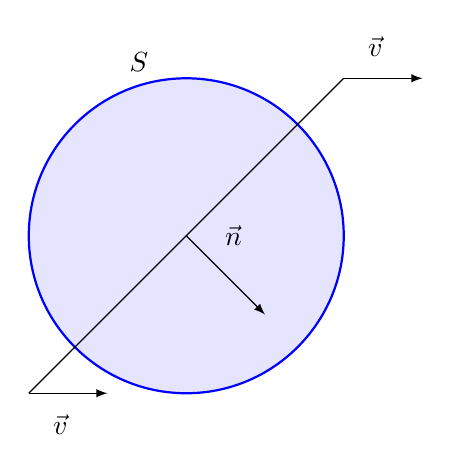
\begin{tikzpicture}[scale=2]
		\draw[thick, blue, fill=blue!10] (0,0) circle(1);
		\draw (-1,-1) -- (1,1);
		\draw[-latex] (-1,-1) -- (-0.5,-1);
		\draw[-latex] (1,1) -- (1.5, 1);
		\draw[-latex] (0,0) -- (0.5,-0.5);
		\node at (1.2,1.2) {$\vec{v}$};
		\node at (-0.8,-1.2) {$\vec{v}$};
		\node at (0.3,-0.0) {$\vec{n}$};
		\node at (-0.3, 1.1) {$\mathfrak{S}$};
	\end{tikzpicture}
	\caption{Aperture problem, figure inspired by \citet{Yazdanbakhsh20111093}. If the line defined by $\vec{n}$ is observed only in the area defined by $\mathfrak{S}$, then any movement along any $\vec{v}$ will be observed as movement along $\vec{n}$.}
	\label{fig:aperture}
\end{figure}

Figure \vref{fig:aperture} tries to illustrate how the aperture problem arises. If the area that are being tracked 
only contains a single edge, then it is impossible to say if there are movement in any direction that is not 
parallel to the normal direction to the edge. This means that tracing a single edge is not favourable, and all 
modern algorithms will try to trace on corners, as a corner by definition is made of at least two non-parallel edges 

\section{Optical flow}
Optical flow is a term that covers the apparent motion of objects, specifically its edges and surfaces 
relative to an observer. The term was first coined for this by James Gibson in the 1940s 
to describe the visual stimulus that animals get from movement in \citet{gibson50}.


\subsection{Theory}
The base of optical flow theory is based on the normal flow constraint equation in \eqref{equ:image.constraint}. In equation \eqref{equ:image.constraint}, $I$ is the intensity
at a given point at a given time. It is quite obvious that a normal optical flow problem will be of three dimension as it will include spatial coordinates in addition
to a temporal part. The deltas shown is an indefinite movement in the three dimensions.


\begin{equation}\label{equ:image.constraint}
	I(x,y,t) = I(x + \Delta x, y+ \Delta y, t + \Delta t)
\end{equation}

If the deltas in equation \eqref{equ:image.constraint} is assumed to be small, then the approximation in equation \eqref{equ:image.constraint.taylor} is valid.

\begin{equation}\label{equ:image.constraint.taylor}
	I(x + \Delta x, y+ \Delta y, t + \Delta t) = I(x,y,t) + \frac{\partial I}{\partial x} \Delta x + 
		\frac{\partial I}{\partial y} \Delta y + \frac{\partial I}{\partial t} \Delta t + \mathcal{O}(\partial^2)
\end{equation}

Equation \eqref{equ:image.constraint.taylor} contains a higher order collection term $\mathcal{O}(\partial^2)$. This can be thought of the error in this first order taylor approximation. As
the deltas are assumed small, then the Taylor expansion terms with order higher than one is negligible. 

Substituting equation \eqref{equ:image.constraint} into \eqref{equ:image.constraint.taylor} it is obvious that equation \eqref{equ:taylor.exp} must hold. 
By dividing equation \eqref{equ:taylor.exp} with the change of time we get \eqref{equ:taylor.exp.subs}, where $V_x$ and $V_y$ are the spatial velocities in the 
$x$ and $y$ direction.

\begin{align}
	\frac{\partial I}{\partial x} \Delta x + \frac{\partial I}{\partial y} \Delta y + 
		\frac{\partial I}{\partial t} \Delta t &= 0 \label{equ:taylor.exp} \\
	\frac{\partial I}{\partial x} \frac{\Delta x}{\Delta t} + \frac{\partial I}{\partial y} \frac{\Delta y}{\Delta t} + 
		\frac{\partial I}{\partial t} \frac{\Delta t}{\Delta t} &= \frac{0}{\Delta t} \notag \\
	\frac{\partial I}{\partial x} V_x + \frac{\partial I}{\partial y} V_y + \frac{\partial I}{\partial t}  &= 0 \label{equ:taylor.exp.subs}
\end{align}

By defining the intensity spatial derivatives as $I_x$, $I_y$ and $I_t$, we get equation \eqref{equ:intensity.deriv}. Using the dot product on the derivatives 
leads to equation \eqref{equ:optical.flow}, which is the usual way of writing the optical flow problem.

\begin{align}
	I_x V_x + I_y V_y &= -I_t \label{equ:intensity.deriv} \\
	\nabla I^\top \cdot \vec{V} &= -I_t \label{equ:optical.flow}
\end{align}

Equation \eqref{equ:optical.flow} shows the big problem of optical flow problems. It is a single equation with two unknowns, and is therefore not 
solvable without adding additional constraints to the analysis. The problem is known as the aperture problem, and all of the following algorithms 
introduces some additional condition that infers constraints to the flow problem.

\subsection{Phase correlation}\label{sec:phase.correlation}
As the name of this method implies, this method uses shift and correlation in the phase plane between to frames as a measure of motion. Given that correlation is a global operation,
the method is also image global. The first step is to apply the Fourier transform to both frames, $\textbf{G}_a = \mathcal{F}\{g_a\}$ and $\textbf{G}_b = \mathcal{F}\{g_b\}$. The cross-power spectrum 
can then be calculated with equation \eqref{equ:phase.cross.power}.

\begin{equation}\label{equ:phase.cross.power}
	R = \frac{\textbf{G}_a \circ \textbf{G}_b^\star}{|\textbf{G}_a \textbf{G}_b^\star|}
\end{equation}

By inverse transforming $R$, we get the normalized cross-correlation, $r = \mathcal{F}^{-1}\{R\}$, which can be though of as a 
heat map of the movement between the two frames.

There are however some drawbacks with using the phase correlation method, in addition to the global aspect. The global aspect 
infers smooth and equal movement of all points between the frames. Also, since the Fourier transform is involved. The method has its base 
in the Fourier shift theorem, which implies that the images are assumed to have a circular shift. The case is, however, that the shift 
is more likely to be linear, and this discrepancy gives distortions in the cross-correlation.

\subsection{Lukas-Kanade}\label{sec:lukas-kanade}
The Lucas-Kanade method is a widely used method for providing the needed constraints to solve \eqref{equ:optical.flow}. This method assumes that 
the motion between to frames is small and more or less constant in the neighbourhood of a point, known as the velocity smoothness constraint. 
This means that \eqref{equ:optical.flow} holds for all points within some window
with the point that is being considered. This means that the local velocity vector should satisfy \eqref{equ:lk.local.flow}.

\begin{equation}\label{equ:lk.local.flow}
	\begin{split}
		I_x(q_1)V_x + I_y(q_1)V_y	&= -I_t(q_1) \\
		I_x(q_2)V_x + I_y(q_2)V_y 	&= -I_t(q_2) \\
		&\,\,\, \vdots \\
		I_x(q_N)V_x + I_y(q_N)V_y 	&= -I_t(q_N)
	\end{split}
\end{equation}

Rewriting \eqref{equ:lk.local.flow} on matrix form using the normal $Av = b$ structure, we get the matrices in \eqref{equ:lk.local.flow.mat}.

\begin{equation} \label{equ:lk.local.flow.mat}
A = \begin{bmatrix}
		I_x(q_1) 	& I_y(q_1) \\
		I_x(q_2) 	& I_y(q_2) \\ 
		\vdots 		& \vdots \\
		I_x(q_N)	& I_y(q_N)
	\end{bmatrix} \quad 
v =	\begin{bmatrix}
		V_x \\ V_y
	\end{bmatrix} \quad
b = \begin{bmatrix}
		-I_t(q_1) \\ -I_t(q_2) \\ \vdots \\ -I_t(q_N)
	\end{bmatrix}
\end{equation}

The equation set in \eqref{equ:lk.local.flow.mat} is overdetermined. The Lucas-Kanade method now uses the 
least squares method to find the minimal solution to this set. The system that then must be solved usually takes the 
form of \eqref{equ:lk.local.flow.solv}.

\begin{equation}\label{equ:lk.local.flow.solv}
	v = \left(A^\top A\right)^{-1} A^\top b
\end{equation}

If equation \eqref{equ:lk.local.flow.solv} is expanded back to its original matrices and using sums, we have the system in \eqref{equ:lk.local.flow.solv.full}

\begin{equation}\label{equ:lk.local.flow.solv.full}
	\begin{bmatrix}
		V_x \\ V_y
	\end{bmatrix} = 
	\begin{bmatrix}
		\sum_ i{I_x^2(q_i)} 	 & \sum_i{I_x(q_i)I_y(q_i)} \\
		\sum_i{I_y(q_i)I_x(q_i)} & \sum{I_y^2(q_i)}
	\end{bmatrix}^{-1}
	\begin{bmatrix}
		-\sum_i{I_x(q_i)I_t(q_i)} \\ -\sum_i{I_y(q_i)I_t(q_i)}
	\end{bmatrix}
\end{equation}

\subsection{Horn-Schunck}\label{sec:horn-schunck}
The Horn-Schunck method is another global algorithm\citet{horn80}. It assumes that the flow in a frame is smooth and will minimize any error in this assumption.
It formulates the flow as a energy function on the form \eqref{equ:horn.schunck}, which can be minimized using the corresponding Euler-Lagrange equations in \eqref{equ:horn.schunck.euler} with
$L=\int{E}$.

\begin{equation}\label{equ:horn.schunck}
	E = \int \int \Big ( \big (I_x u + I_y v + I_t\big )^2 + \alpha^2\big (||\nabla u||^2 + ||\nabla v||^2\big ) \Big )\; \mathrm{d}x\,\mathrm{d}y
\end{equation}

\begin{equation}\label{equ:horn.schunck.euler}
	\begin{split}
		\frac{\partial L}{\partial u} - \frac{\partial}{\partial x}\frac{\partial L}{\partial u_x} - \frac{\partial}{\partial y}\frac{\partial L}{\partial u_y} &= 0 \\
		\frac{\partial L}{\partial v} - \frac{\partial}{\partial x}\frac{\partial L}{\partial v_x} - \frac{\partial}{\partial y}\frac{\partial L}{\partial v_y} &= 0
	\end{split}
\end{equation}

The solution to the system in \eqref{equ:horn.schunck} and \eqref{equ:horn.schunck.euler} uses the same arguments as those given in \citet{khalil01} for energy based system analysis.
The full analytical steps and solution can be found in \citet{horn80} which will be omitted here. The result usually takes the form as the iterative equations in \eqref{equ:horn.schunck.solution}.

\begin{equation}\label{equ:horn.schunck.solution}
	\begin{split}
		u^{k + 1} &= \bar{u}^k - \frac{I_x\left(I_x\bar{u}^k + I_y\bar{u}^k + I_t\right)}{\alpha^2 + I_x^2 + I_y^2} \\
		v^{k + 1} &= \bar{v}^k - \frac{I_x\left(I_x\bar{v}^k + I_y\bar{v}^k + I_t\right)}{\alpha^2 + I_x^2 + I_y^2}
	\end{split}
\end{equation}

